\subsection{Offsetjustering}
\subsubsection{Teori og design}
Det analoge signal der kommer fra accelrometeret har et indbygget offset på halvdelen af dens spændingsforsyning. For at kunne forstærke signalet der båder skal indholde positive og negative værdier, er det nødvendigt at fjerne dette offset. På denne måde vil accelerometeret i steady state have et outputsignal på $0$V. Måden dette offset indføres er ved anvendelse af et differensforstærker kredsløb. Dette kredsløb kan tage et af inputsignalerne og minusse det med det andet inputsignal. Kredsløbet designes således:

\begin{figure}[H]
\centering
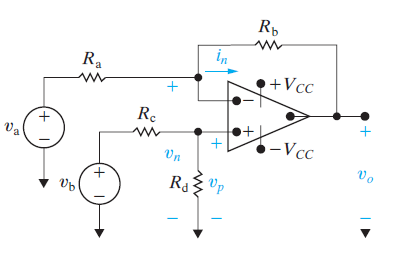
\includegraphics[scale=1]{figures/cProblemloesning/Differensforstaerker_generisk.png}
\caption{På figuren er et generisk differensforstærker kredsløb illustreret.}
\label{fig:Differensforstaerker_generisk}
\end{figure}

Ligning \ref{eq:Diff1} er den simplificeret ligning for differensforstærker kredsløbet, hvor $\frac{R_a}{R_b} = \frac{R_c}{R_d}$.

\begin{equation}\label{eq:Diff1}
V_o = \frac{R_b}{R_a} \cdot (v_b - v_a)
\end{equation}

Det kan heraf ses at forstærkningen på signalet kan bestemmes ved at vælge modstandene $R_a \text{og} R_b$ og at det er spændingsforsyningen $v_a$ der trækkes fra spændingsforsyningen $v_b$. 

I dette tilfælde kræves der ikke en forstærkning, derfor skal modstandene $R_a \text{og} R_b$ være det samme. Da signalet ikke skal inverteres sættes accelerometerets output ind i den ikke-inverterende kanal? og offsettet, som i dette tilfælde er på $1.5915$V ind i den inverterende kanal?. Dette illustreres på figur \ref{fig:Offset_generisk}:
\begin{figure}[H]
\centering
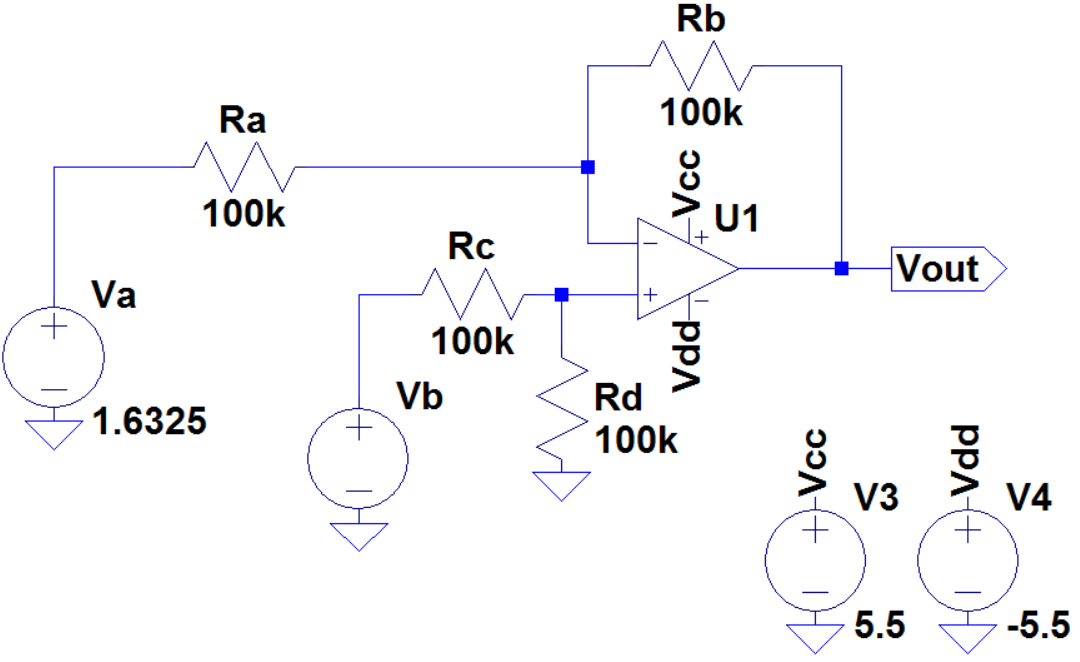
\includegraphics[scale=1]{figures/cProblemsloesning/Offset_generisk.png}
\caption{•}
\label{fig:Offset_generisk}
\end{figure}

Grunden til at spændingsforsyningen er $\pm 6$V er at spændingsforsyningen til hele systemet, er designet til at give et output på $\pm 6$V. 